\newcommand{\lorentz}{\mathcal{L}}
\newcommand{\lorentzpropio}{\mathcal{L}_+}
\newcommand{\lorentzorto}{\mathcal{L}^\uparrow}
\newcommand{\lorentzortopropio}{\mathcal{L}_+^\uparrow}
\newcommand{\SL}{\mathrm{SL}(2,\mathbb{C})}

\section{El grupo de Lorentz}

% \begin{definicion}
El espacio de Minkowski es un espacio $\mathbb{R}^4$ con una métrica pseudo-euclídea de signatura $(+,-,-,-)$. En una base en la que los 4-vectores $x^\mu$ (contravariantes) tienen coordenadas $(x^\mu)=(x^0,x^1,x^2,x^3)=(ct,x,y,z)=(x^0,\vec{x})$ la métrica es diagonal 
\begin{equation}
\eta_{\mu\nu}=\operatorname{diag}(1,-1,-1,-1)
\end{equation}
y la norma al cuadrado del 4-vector es
\begin{equation}
x\cdot x=x^\mu \eta_{\mu\nu} x^\nu=(x^0)^2-\vec{x}^2
\end{equation}

El \textbf{grupo de Lorentz} $\lorentz\cong \mathrm{O}(1,3)$ es el grupo de isometría de esta forma cuadrática, es decir
\begin{flalign}
\Lambda\in \mathrm{O}(1,3):\quad &x\xrightarrow{\Lambda} x'=\Lambda x\qquad x^{\prime\mu}=\Lambda^\mu_{\ \nu}\  x^\nu \label{transf_coords_4_vector}\\
&x'\cdot x'=\Lambda^\mu_{\ \rho}\ x^\rho\ \eta_{\mu\nu}\ \Lambda^\nu_{\ \sigma}\ x^\sigma  =x\cdot x\\
\therefore\quad & \boxed{\Lambda^\mu_{\ \rho}\ \eta_{\mu\nu}\ \Lambda^\nu_{\ \sigma}=\eta_{\rho\sigma}}\qquad \boxed{\Lambda^t\ \eta\ \Lambda=\eta} \label{ec_isometria}
\end{flalign}
\medskip 

\begin{itemize}
\item $\lorentz$ es un grupo de Lie lineal de dimensión 6: $\Lambda^\mu_{\ \nu}$ son 16 componentes sujetas a 10 ecuaciones.
\item $\lorentz$ es un grupo no conexo, formado por 4 conjuntos disjuntos (componentes u hojas). En efecto, de \eqref{ec_isometria} se sigue
% \begin{flalign}
\begin{gather}
\det \Lambda^t\ \det\Lambda=(\det\Lambda)^2 =1\Longrightarrow  \det \Lambda=\pm1\\
\Lambda^\mu_{\ 0}\ \eta_{\mu\nu}\ \Lambda^{\nu}_{\ 0}=(\Lambda^0_0)^2-\sum_i(\Lambda^i_0)^2=1\Rightarrow \Lambda^0_{\ 0}=\left\{\begin{aligned}
&\geq\enskip\  1\\
&\leq -1
\end{aligned}	\right.
% \end{flalign}
\end{gather}
\end{itemize}
% \end{definicion}

Cada una de estas componentes sí es conexa. Nos restringiremos a la componente conectada con la identidad, llamada \textbf{subgrupo ortocrono propio} o \textbf{grupo de Lorentz restringido}: $\lorentzortopropio\cong \mathrm{SO}(1,3)$. \medskip

Todas las $\Lambda\in\lorentzortopropio$ pueden escribirse como el producto de una rotación $R\in \SO$ por una <<transformación de Lorentz pura>> o \emph{boost} $L$.

\begin{flalign}
R_{\normalv}(\phi)&=\left(\begin{array}{c|c}
1&\\
\hline
&{R_{\normalv}(\phi)}{\in\SO}
\end{array}\right) \label{rotacion_lorentz}\\
L_1&=\begin{pmatrix}
\gamma&-\beta \gamma &0&0\\
-\beta \gamma& \gamma &0&0\\
0&0&1&0\\
0&0&0&1
\end{pmatrix}=\begin{pmatrix}
\cosh\psi&-\sinh\psi&0&0\\
-\sinh\psi& \cosh\psi &0&0\\
0&0&1&0\\
0&0&0&1
\end{pmatrix}\qquad \gamma=:\cosh\psi\\
L&=(L^\mu_{\ \nu})=\left(\begin{array}{c|c}
\cosh\psi&n_j\sinh \psi\\
\hline
-n^i\sinh\psi&\delta^i_{\ j}-n^in_j\ (\cosh\psi-1)
\end{array}\right) = \left(\begin{array}{c|c}
\gamma&\beta_j\gamma\\
\hline
-\beta^i\gamma&\delta^i_{\ j}-\frac{\beta^i\beta_j}{\beta^2}\ (\gamma-1)
\end{array}\right)
\end{flalign}
con $\vec{n}=(n^1,n^2,n^3)$ vector unitario en la dirección $\vec{\beta}=\vec{v}/c$. \medskip

De \eqref{rotacion_lorentz} se sigue que $\SO$ es subgrupo de $\lorentzortopropio$.

\begin{remark}
Las transformaciones de Lorentz puras en general no forman subgrupo, solo las que son uniparamétricas como $L_1$.
\end{remark}


\begin{flushleft}
\textbf{Parametrización.} Una transformación genérica $\Lambda\in \lorentzortopropio$ se puede obtener (como mostraremos más adelante) de la forma $\Lambda=LR$.
\end{flushleft}

De los 6 parámertros que caracterizan $\Lambda$, podemos asociar 3 a los 3 parámetros de $R$ y otros 3 a los de $L$. El espacio de parámetros correspondiente a la transformación $L$ se puede tomar como un hiperboloide en el espacio euclídeo de dimensión 4. De hecho, la cantidad
\begin{equation}
x\cdot x=(x^0)^2-(\vec{x})^2=\text{const.}
\end{equation}
(ec. del hiperboloide) es invariante bajo $L$.


%dibujico hiperboloide
\begin{figure}[ht]
    \centering
    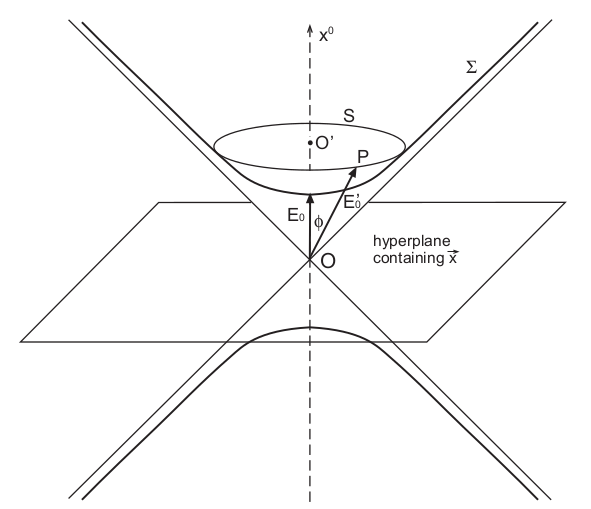
\includegraphics[width=  0.4\linewidth]{hyperboloid_boosts.png}
    \caption[Dominio de la parametrización para las transformaciones de Lorentz puras]{Dominio de la parametrización para las transformaciones de Lorentz puras \footnotemark}
    \label{fig:hiperboloide_boosts}
\end{figure}


El hiperboloide tiene dos ramas dentro del cono de luz, pero si consideramos $x^0>0$ solo necesitamos la primera ($\Sigma$), ya que $L\in\lorentzortopropio$ no puede cambiar el signo de $x^0$. Un \emph{boost} $L:E_0\rightarrow E_0'$ queda unívocamente definido por el punto $P$. Para un $\phi$ dado, $P$ se encuentra en la esfera $S$ (un círculo en la figura \ref{fig:hiperboloide_boosts}) y necesitamos dos parámetros más para fijar la posición de $P$ en $S$. En el espacio de Minkowski $\phi$ se convierte en imaginario, y corresponde a $\psi=i\phi$. \medskip

\footnotetext {Giovanni Costa, Gianluigi Fogli, \emph{Symmetries and Group Theory in Particle Physics} p. 48}


Las propiedades topológicas de este espacio de parámetros nos permiten inferir las siguientes propiedades de $\lorentzortopropio$:
\begin{itemize}
\item $\lorentzortopropio$ es un grupo\textbf{no compacto}, al no ser compacto el hiperboloide.
\item $\lorentzortopropio$ es \textbf{doblemente conexo}. El subconjunto de los \emph{boosts} $L$ es simplemente conexo, puesto que cualquier camino cerrado en $\Sigma$ se puede deformar de forma continua a un punto. Sin embargo, como ya vimos, el subgrupo $\SO$ de las rotaciones es doblemente conexo, y por tanto lo es el propio $\lorentzortopropio$. 
\end{itemize} 

\begin{flushleft}
\textbf{Recubridor universal} de $\lorentzortopropio \cong\mathrm{SO}(1,3)$: grupo simplemente conexo homeomorfo a 
$\lorentzortopropio$. 
\end{flushleft}

Asociamos a cada 4-vector la matriz hermítica
\begin{equation}
X=\sigma_\mu x^\mu =\begin{pmatrix}
x^0+x^3& x^1-ix^2\\
x^1+ix^2&x^0-x^3
\end{pmatrix}\label{matriz_X_Lorentz}
\end{equation}
con $\sigma_\mu:=(\sigma_0,\vec{\sigma}),\qquad\sigma^\mu\equiv \underline{\sigma}_\mu:=(\sigma_0,-\vec{\sigma}),\qquad\sigma_0:=\mathbb{1}_{2\times 2}$. \medskip

% \begin{gather}
% \sigma_\mu:=(\sigma_0,\vec{\sigma})\\
% \sigma^\mu\equiv \underline{\sigma}_\mu:=(\sigma_0,-\vec{\sigma})\\
% \sigma_0:=\mathbb{1}_{2\times 2}
% \end{gather}

Se verifica
\begin{gather}
\trace{\underline{\sigma}_\mu \sigma_\nu}=2\eta_{\mu\nu}\\
x^\mu=\frac{1}{2}\trace{\underline{\sigma}^\mu X}
\end{gather}

% Nótese que $\det X=x\cdot x$

Introducimos una matriz compleja unimodular
\begin{equation}
A=\begin{pmatrix}
\alpha &\beta \\
\gamma &\delta
\end{pmatrix}  \quad \text{con}\quad \det A=\alpha\delta-\beta\gamma=1
\label{matrices_A_Lorentz}
\end{equation}
% con $\det A=1$,
 y transformemos $X$ según
\begin{equation}
X'=AXA^\dagger\Rightarrow x'\cdot x'=\det X'=\det X= x\cdot x
\end{equation}

$A$ describe una transformación lineal de $x^\mu$ que deja $x\cdot x$ invariante, esto es, una transformación de Lorentz. La relación entre matrices $A$ y $\Lambda$ está dada por
\begin{gather}
\Delta^\mu_{\ \nu}\  x^\nu= x'\mu=\frac{1}{2} \trace{\underline{\sigma}^\mu X'}= \frac{1}{2}\trace{\underline{\sigma}^\mu A \sigma_\nu A^\dagger }\ x^\nu \\
\therefore \Lambda^\mu_{\ \nu}= \frac{1}{2}\trace{\underline{\sigma}^\mu A \sigma_\nu A^\dagger }
\end{gather}


El conjunto de matrices $A$ dadas por \eqref{matrices_A_Lorentz} forman el grupo $\mathrm{SL}(2,\mathbb{C})$. Por cada matriz $A$ hay una transformación de Lorentz $\Lambda$, y por cada transformación de Lorentz $\Lambda$ hay dos matrices de $\SL$: $A$ y $-A$. En particular, tanto $\mathbb{1}$ como $-\mathbb{1}$ se corresponden con la identidad en $\lorentzortopropio$. Esta relación entre $\SL$ y $\lorentzortopropio$ es un homomorfismo, ya que preserva la estructura de grupo. \medskip

Podemos escribir $A=e^S$, con $S$ una matriz $2\times 2$ de traza nula. Hay 6 matrices $2\times 2$ sin traza que sean independientes, podemos elegir las 3 matrices de Pauli hermíticas $\sigma_k$ y las tres matrices anti-hermíticas $i\sigma_k$. Entonces, en general, $S=S_1+S_2$ con
\begin{flalign}
&S_1=-i\frac{\phi}{2}\vec{n}\cdot\vec{\sigma}\\
&S_2=-\frac{\psi}{2}\vec{u}\cdot \vec{\sigma}
\end{flalign} 
donde $\phi$ y $\psi$ son parámetros reales y $\vec{n}$ y $\vec{u}$ vectores unitarios reales. \medskip

Obtenemos \underline{dos tipos de matrices: unitarias y hermíticas}.
\begin{flalign}
& U=e^{S_1}=\cos\left(\frac{\phi}{2}\right)\mathbb{1}-i\sin\left(\frac{\phi}{2}\right) \vec{n}\cdot \vec{\sigma}\in \SU\subset\SL\\
&H=e^{S_2}=\cosh \left(\frac{\psi}{2}\right)\mathbb{1}-i\sinh\left(\frac{\psi}{2}\right) \vec{u}\cdot \vec{\sigma}
\end{flalign}
que corresponden a rotaciones puras y a \emph{boosts} puros (con $\vec{\beta}=\vec{u}\tanh \psi$) respectivamente. \medskip

Un teorema de álgebra lineal garantiza que toda matriz $A\in\SL$ se puede escribir como $A=HU$. El homomorfismo entre $\SL$ y $\lorentzortopropio$ implica
\begin{equation}
\Lambda(A)=\Lambda(H)\Lambda(U)\Longrightarrow \boxed{\Lambda=LR}
\end{equation}

\begin{flushleft}
\textbf{Álgebra de Lie} de $\lorentzortopropio$. Como ya sabemos, las transformaciones infinitesimales se corresponden con los generadores del álgebra.
\end{flushleft}
El subgrupo de las rotaciones espaciales puras es generado por tres elementos independientes, que escogemos $R_1(\phi),\ R_2(\phi)$ y $R_3(\phi)$ (vistas como matrices $4\times 4$. 
\begin{equation}
\left(\begin{array}{c|c}
1&\\
\hline
& R_i(\phi)_{3\times3 }
\end{array}\right)
\end{equation}

Los generadores hermíticos de estas rotaciones son
\begin{gather}
J_k=i\left.\parder{R_k}{\phi}\right|_{\phi=0}\qquad k=1,2,3\\
\left(\begin{array}{c|c}
0&\\
\hline
& (J_i)_{\SO}
\end{array}\right)\\
J_{1}=\left(\begin{array}{cccc}{0} & {0} & {0} & {0} \\ {0} & {0} & {0} & {0} \\ {0} & {0} & {0} & {-i} \\ {0} & {0} & {i} & {0}\end{array}\right), \quad J_{2}=\left(\begin{array}{cccc}{0} & {0} & {0} & {0} \\ {0} & {0} & {0} & {i} \\ {0} & {0} & {0} & {0} \\ {0} & {-i} & {0} & {0}\end{array}\right), \quad J_{3}=\left(\begin{array}{cccc}{0} & {0} & {0} & {0} \\ {0} & {0} & {-i} & {0} \\ {0} & {i} & {0} & {0} \\ {0} & {0} & {0} & {0}\end{array}\right)
\end{gather}

Una rotación infinitesimal pura (de ángulo $\delta\phi$) viene dada por
\begin{equation}
R=\mathbb{1}-i\delta\phi\vec{n}\cdot\vec{J}
\end{equation}


Análogamente, podemos derivar los generadores infinitesimales anti-hermíticos $K_l$ de los \emph{boosts} a partir del conjunto linealmente independiente $\{L_1(\psi),L_2(\psi),L_3(\psi)\}$

\begin{gather}
K_l=i\left. \parder{L_l}{\psi}\right|_{\psi=0}\qquad l=1,2,3\\
K_{1}=\left(\begin{array}{cccc}{0} & {-i} & {0} & {0} \\ {-i} & {0} & {0} & {0} \\ {0} & {0} & {0} & {0} \\ {0} & {0} & {0} & {0}\end{array}\right), K_{2}=\left(\begin{array}{cccc}{0} & {0} & {-i} & {0} \\ {0} & {0} & {0} & {0} \\ {-i} & {0} & {0} & {0} \\ {0} & {0} & {0} & {0}\end{array}\right), K_{3}=\left(\begin{array}{cccc}{0} & {0} & {0} & {-i} \\ {0} & {0} & {0} & {0} \\ {0} & {0} & {0} & {0} \\ {-i} & {0} & {0} & {0}\end{array}\right)
\end{gather}

Un \emph{boost} infinitesimal puro (de rapidez $\delta\psi$) a lo largo de la dirección $\vec{n}$ está dado por
\begin{equation}
L=\mathbb{1}-i\delta\psi \vec{u}\cdot \vec{K}\qquad \vec{u}=\frac{\vec{v}}{\abs{\vec{v}}}
\end{equation}

Las transformaciones finitas se obtienen de exponenciar el álgebra\footnote{Aunque formalmente $\Lambda=LR$, la $\Lambda$ dada por \eqref{Lorentz_general_finita} NO es el producto de la $L$ dada por \eqref{boost_finito} por la $R$ dada por \eqref{rotacion_finita}.}
\begin{flalign}
&R=e^{-i\phi \vec{n}\cdot \vec{J}} \label{rotacion_finita}\\
&L=e^{-i\psi \vec{u}\cdot \vec{K}} \label{boost_finito}\\
&\Lambda= e^{-i(\phi \vec{n}\cdot \vec{J}+\psi \vec{u}\cdot \vec{K})} \label{Lorentz_general_finita}
\end{flalign}

El álgebra de Lie de $\lorentzortopropio$ y dde $\SL$ cumple las  \textbf{reglas de conmutación} siguientes
\begin{subequations}
\begin{flalign}
\left[J_{i}, J_{j}\right] &=i \epsilon_{i j k} J_{k} \\\left[K_{i}, K_{j}\right] &= - i \epsilon_{i j k} J_{k} \\\left[J_{i}, K_{j}\right] &=i \epsilon_{i j k} K_{k} 
\end{flalign}
\label{conmutadores_lorentz}
\end{subequations}

Definimos el tensor antisimétrico $M_{\mu\nu}$ de componentes
\begin{flalign}
&\left(M_{12}, M_{23}, M_{31}\right)=\left(J_{3}, J_{1}, J_{2}\right) \longrightarrow M_{ij}=\epsilon_{ijk}J_k\\ 
&\left(M_{01}, M_{02}, M_{03}\right)=\left(K_{1}, K_{2}, K_{3}\right)\longrightarrow M_{0i}=K_i=-M_{i0}
\end{flalign}

de modo que los conmutadores \eqref{conmutadores_lorentz} en forma covariante resultan
\begin{equation}
\left[M_{\lambda \rho}, M_{\mu \nu}\right]=-i\left(\eta_{\lambda \mu} M_{\rho \nu}+\eta_{\rho \nu} M_{\lambda \mu}-\eta_{\lambda \nu} M_{\rho \mu}-\eta_{\rho \mu} M_{\lambda \nu}\right)
\end{equation}
y una transformación general de $\lorentzortopropio{}$ se puede escribir como
\begin{equation}
\Lambda=e^{-\frac{1}{2} i \omega^{\mu \nu} M_{\mu \nu}}
\end{equation}
donde $\omega^{\mu\nu}$ es una matriz real antisimétrica. \medskip

Se tienen los dos \textbf{Casimires}
\begin{flalign}
 \frac{1}{2} M^{\mu \nu} M_{\mu \nu} &=\vec{J}^{2}-\vec{K}^{2} \\ 
 \frac{1}{2} \epsilon^{\mu \nu \sigma \tau} M_{\mu \nu} M_{\sigma \tau} &=-\vec{J} \cdot \vec{K} 
\end{flalign}


\begin{flushleft}
\textbf{Representaciones irreducibles de} $\lorentzortopropio\cong\mathrm{SO}(1,3)$. Al ser $\lorentzortopropio$ no compacto, dichas representaciones no pueden ser unitarias. Al no ser hermíticos los generadores $\vec{K}$, las matrices $\Lambda$ en general no serán unitarias.
\end{flushleft}

Para clasificar las representaciones irreducibles introducimos las siguientes combinaciones de generadores
\begin{subequations}
\begin{flalign}
M_{i}=\frac{1}{2}\left(J_{i}+i K_{i}\right)\\
N_{i}=\frac{1}{2}\left(J_{i}-i K_{i}\right)
\end{flalign}
\end{subequations}
 que son hermíticas. Cumplen las reglas de conmutación
\begin{flalign}
&\left[M_{i}, M_{j}\right]=i \epsilon_{i j k} M_{k}\\
&\left[N_{i}, N_{j}\right]=i \epsilon_{i j k} N_{k}\\
&\left[M_{i}, N_{j}\right]=0
\end{flalign}

$\vec{M}$ y $\vec{N}$ son los generadores de dos copias de $\su_{\mathbb{C}}$ ($\su$ complejificado). Es decir, si denotamos por $M_{\mathbb{C}}$ y $N_{\mathbb{C}}$ la envolvente lineal compleja de $\vec{M}$ y $\vec{N}$ tenemos el isomorfismo
\begin{equation}
\mathfrak{so}(1,3)_{\mathbb{C}}=M_{\mathbb{C}}\ \oplus\ N_{\mathbb{C}}\cong \su_{\mathbb{C}}\ \oplus\ \su_{\mathbb{C}}\cong \mathfrak{sl}(2,\mathbb{C})\ \oplus\ \mathfrak{sl}(2,\mathbb{C})
\end{equation}

Tenemos que
\begin{subequations}
\begin{flalign}
&[\vec{M}^2,M_i]=0\\
&[\vec{N}^2,N_i]=0
\end{flalign}
\end{subequations}
por lo que podemos etiquetar las representaciones irreducibles de $\lorentzortopropio$ con los autovalores $j(j+1)$ y $j'(j'+1)$ de los Casimir $\vec{M}^2$ y $\vec{N}^2$ respectivamente, donde $j,j'=0,1/2,1,3/2,\ldots$\medskip


 Podemos tomar los $d=(2j+1)(2j'+1)$ autoestados independientes como base del EV sobre el que actúa la representación irreducible de dimensión $d$ de $\lorentzortopropio$. Cada elemento $\Lambda\in\lorentzortopropio$ queda representado por una matriz $D^{(j,j')}(\Lambda)$. \bigskip

Restringiéndonos al subgrupo de rotaciones $\SO$, las representaciones dejan de ser irreducibles y pueden descomponerse en términos de las representaciones irreducibles de $\SO$ de la forma

\begin{equation}
D^{\left(j, j^{\prime}\right)}(R)=D^{(j)}(R) \otimes D^{\left(j^{\prime}\right)}(R)=D^{\left(j+j^{\prime}\right)}(R) \oplus \ldots \oplus D^{\left(\left|j-j^{\prime}\right|\right)}(R)
\end{equation}

Al igual que para $\SO$ se tienen dos clases de representaciones irreducibles para $\lorentzortopropio$: tensoriales y espinoriales, con $j+j'$ entero y semi-entero respectivamente. Las espinoriales se obtienen de su recubridor universal $\SL$ y desde el punto de vista de $\lorentzortopropio$ son bivaluadas --al ser $\lorentzortopropio$ doblemente conexo, sus elementos admiten dos representaciones de $\SL$. Mientras que los campos tensoriales se transforman bien  bajo $\mathrm{SO}(1,3)$, los campos espinoriales se transforman bajo $\SL$, análogamente a los tensores y espinores de $\SO$ y $\SU$.

\begin{flushleft}
\textbf{Representaciones de espín más bajo}. Hay dos representaciones de dimensión 2 inequivalentes: $D^{(\frac{1}{2},0)}$ y $D^{(0,\frac{1}{2})}$
\end{flushleft}

Mientras que $\Lambda(A)=\Lambda(-A)$, $A$ y $\bar{A}$ no dan lugar a representaciones equivalentes. Como en general las matrices $A\in \SL$ no son unitarias, no hay una transformación de similaridad que relacione $A$ con $\bar{A}$. En el caso de las rotaciones, una representación y su compleja conjugada sí que son equivalentes.\medskip

Las matrices $A$ y $\bar{A}$ constituyen, en general, dos representaciones irreducibles inequivalentes de $\lorentzortopropio$ que actúan en dos espacios vectoriales diferentes. Tenemos entonces dos bases no equivalentes y, generalmente, dos clases de biespinores (contravariantes): $\xi$ y $\overline{\xi}$.\medskip

Estos biespinores se transforman de acuerdo a 

\begin{subequations}
\begin{flalign}
&\xi'=A\xi \qquad \text{en comps. contravariantes:  } \xi= \begin{pmatrix}
\xi^1 \\ \xi^2
\end{pmatrix}\quad \xi^{\prime\alpha}=A^\alpha_{\ \beta} \xi^\beta\quad \alpha,\beta=1,2\\
&\bar{\xi}'=\bar{A}\bar{\xi} \qquad \text{en comps. contravariantes:  } \bar{\xi}= \begin{pmatrix}
\xi^{\dot{1}} \\ \xi^{\dot{2}}
\end{pmatrix}\quad  \bar{\xi}^{\prime\dot{\alpha}}=\bar{A}{\dot{\alpha}}_{\ \dot{\beta}} \xi^{\dot{\beta}}\quad \alpha,\beta=1,2
\end{flalign}
\end{subequations}

En términos de componentes covariantes $\eta=\left(\eta_{1} \quad \eta_{2}\right), \bar{\eta}=\left(\eta_{\mathrm{i}} \quad \eta_{\dot{2}}\right)$
\begin{subequations}
\begin{flalign}
&\eta_{\alpha}^{\prime}=\eta_{\beta}\left(A^{-1}\right)_{\alpha}^{\beta} \Longleftrightarrow \eta'=\eta A^{-1}\\
&\eta_{\dot{\alpha}}^{\prime}=\eta_{\dot{\beta}}\left(\bar{A}^{-1}\right)_{\dot{\alpha}}^{\dot{\beta}}\Longleftrightarrow \bar{\eta}'=\bar{\eta}A^\dagger
\end{flalign}
\end{subequations}
y los productos $\eta\xi$ y $\bar{\eta} \bar{\xi}$ son invariantes (escalares bajo $\lorentzortopropio$). \medskip


Queremos obtener los generadores $\vec{J}$ y $\vec{K}$ para las representaciones $A$ y $\bar{A}$. Sabemos que 
\begin{gather}
A=e^{-\frac{i}{2}(\phi \vec{n}\cdot \vec{\sigma}-i\psi \vec{u}\cdot\vec{\sigma})}\\
A=e^{-\frac{i}{2}(-\phi \vec{n}\cdot \vec{\sigma}^*-i\psi \vec{u}\cdot\vec{\sigma}^*)}\\
D=e^{-i(\phi \vec{n}\cdot \vec{J}+\psi \vec{u}\cdot \vec{K})}
\end{gather}
de modo que
\begin{itemize}
\item Para los espinores $\xi\quad J_i=\frac{1}{2}\sigma_i,\ K_i=-\frac{i}{2}\sigma_i\Longrightarrow M_i=\frac{\sigma_i}{2},\enskip N_i=0\leadsto j=\frac{1}{2},\enskip j'=0\longrightarrow D^{\left(\frac{1}{2},0\right)}(\Lambda)$
\item Para los espinores $\bar{\xi}\quad J_i=-\frac{1}{2}\sigma_i,\ K_i=-\frac{i}{2}\sigma_i$. Como $\sigma_2\sigma_i^*\sigma_2=-\sigma_i$, esta representación es equivalente a $S_i=\frac{1}{2}\sigma_i,\enskip K_i=\frac{i}{2}\sigma_i\Longrightarrow M_i=0,\enskip N_i=\frac{\sigma_i}{2}\leadsto j=0,\enskip j'=\frac{1}{2}\longrightarrow D^{\left(0,\frac{1}{2}\right)}(\Lambda)$
\end{itemize}

$A$ y $(A^t)^{-1}$ están relacionadas por una transformación de similaridad, de modo que corresponden a representaciones equivalentes:
\begin{equation}
\exists C\in\SL \text{ tal que } (A^t)^{-1}=CAC^{-1}\Leftrightarrow C=A^tCA 
\end{equation}

En particular, para $C=i\sigma_2$ se tiene
\begin{equation}
\tilde{\eta}^{\prime}=\tilde{A}^{-1} \tilde{\eta}=C A C^{-1} \tilde{\eta}\Longrightarrow\tilde{\eta}=C \xi
\end{equation}

\begin{flushleft}
\textbf{Representación de dimensión 4: $D^{\left(\frac{1}{2},\frac{1}{2}\right)}$}. El EV es el de los 4-vectores $x^\mu$ que se transforman de acuerdo con \eqref{transf_coords_4_vector} o \eqref{matriz_X_Lorentz}. Consideremos la cantidad $\xi\bar{\xi}$ que se transforma según
\end{flushleft}
\begin{equation}
\xi'\xi^{\prime\dagger} =A\xi\xi^\dagger A^\dagger
\end{equation}
al igual que $X'$. \medskip

Es decir que podemos tomar $\xi\xi^\dagger$ como la base del espacio de representación $D^{\left(\frac{1}{2},\frac{1}{2}\right)}$. Esto es consistente con
\begin{equation}
D^{\left(\frac{1}{2},\frac{1}{2}\right)}=\underbrace{D^{\left(\frac{1}{2},0\right)}}_\xi \otimes \underbrace{D^{\left(0,\frac{1}{2}\right)}}_{\bar{\xi}}
\end{equation}
y por tanto debe contener los dos tipos de espinores $\xi$ y $\bar{\xi}$.


\begin{nota}
Si queremos mantener la correspondencia entre representaciones irreducibles y estados de espín bien definido para $\lorentzortopropio$ (al igual que para $\SO$) tenemos que introducir condiciones extra que reduzcan el número de elementos independientes de la base. En particular, una partícula de espín 1 se describe con una base de 4 dimensiones, por lo que necesitamos una condición extra para dejar solo 3 elementos independientes, llamada condición de Lorentz:
\begin{equation}
\partial_\mu A^\mu (x)=0
\end{equation}
(para fotones).
\end{nota} 


\begin{flushleft}
\textbf{Transformación de funciones escalares.} El espacio de funciones $\psi(x)$ con $x=(x^0,x^i)=(ct,-x_i)$ proporciona una representación de los operadores $X_\mu,\ P_\mu$ y $M_{\mu\nu}$:
\end{flushleft}
\begin{flalign}
&X_\mu \psi(x)=x_\mu \psi(x)\\
&P_\mu \psi(x)=\textcolor{red} {+} i\partial_\mu \psi(x) \label{momento_lorentz}\\
& M_{\mu\nu}=X_{\mu}P_{\nu} -X_{\nu}P_{\mu}
\end{flalign}
donde el signo positivo en \eqref{momento_lorentz} proviene de la signatura $(+,-,-,-)$.\medskip

Para una transformación de Lorentz infinitesimal
\begin{flalign}
 \delta x^\mu &=x^{\prime\mu}-x^\mu=-\frac{i}{2} \delta\omega^{\rho\sigma} (M_{\rho\sigma})^\mu_{\ \nu}\ x^\nu\\
 \delta \psi(x)&=\psi'(x)-\psi(x)=\psi'(x'-\delta x)-\psi(x)=-\delta x^\mu \partial_\mu \psi(x)\nonumber \\
 &=\frac{i}{2} \delta\omega^{\rho\sigma} (M_{\rho\sigma})^\mu_{\ \nu}\ x^\nu\parder{}{x^\mu} \psi(x)\equiv -\frac{i}{2} \delta\omega^{\rho\sigma} \tilde{M}_{\rho\sigma}(\psi)
\end{flalign}
con
\begin{flalign}
&(M_{\rho\sigma})^\mu_{\ \nu}=i\left(\eta_{\rho}^{\ \mu}\eta_{\sigma\nu} - \eta_{\sigma}^{\ \mu}\eta_{\rho\nu}\right)\\
&\tilde{M}_{\rho\sigma}=-i\left(\eta_{\rho}^{\ \mu}\eta_{\sigma\nu} - \eta_{\sigma}^{\ \mu}\eta_{\rho\nu}\right)x^\nu \parder{}{x^\mu}=-i \left(x_\sigma \parder{}{x^\rho}-x_\rho \parder{}{x^\sigma} \right)= X_\rho P_\sigma -X_\sigma P_\rho
\end{flalign}

\newpage
\begin{flushleft}
\textbf{Espinor de Weyl levógiro.} Campo $\psi_L(x)$ que bajo $\Lambda$ se transforma en la representación $\left(\frac{1}{2},0\right)$, es decir se transforma según
\end{flushleft}
\begin{equation}
\psi_L(x)\xrightarrow{\Lambda}  \psi_L'(x')=\underbrace{e^{(-i\phi \vec{n}-\psi \vec{u})\cdot \frac{\vec{\sigma}}{2}}  }_{\Lambda_L}\ \psi_L(x)
\end{equation}
con
\begin{equation}
\Lambda_L=e^{(-i\phi \vec{n}-\psi \vec{u})\cdot \frac{\vec{\sigma}}{2}}   \label{lambda_Weyl_A}
\end{equation}

Veamos la representación de los generadores de Lorentz sobre $\psi_L$
\begin{flalign}
\delta \psi_L(x)&=\psi_L'(x)-\psi_L(x)=\psi_L'(x'-\delta x)-\psi_L(x)=\nonumber \\
&=\underbrace{\psi'_L(x')}_{\Lambda_L\psi_L(x)}-\delta x^\mu \parder{}{x^\mu} \psi(x)-\psi_L(x)=(\Lambda_L-\Lambda)\psi_L(x)-\delta x^\mu \parder{}{x^\mu} \psi(x)
\end{flalign}

Escribiendo $\Lambda_L$ de la forma
\begin{equation}
\Lambda_L=e^{-\frac{i}{2}\delta \omega^{\mu\nu}\tilde{S}_{\mu\nu}}=1-\frac{i}{2}\delta \omega^{\mu\nu}\tilde{S}_{\mu\nu} \label{lambda_Weyl_B}
\end{equation}
se tiene
\begin{equation}
\delta \psi_L=-\frac{i}{2}\delta \omega^{\mu\nu}\tilde{J}_{\mu\nu}\psi_L
\end{equation}
con $\tilde{J}_{\mu\nu}$ el momento angular total:
\begin{equation}
\tilde{J}_{\mu\nu}=\tilde{M}_{\mu\nu}+\tilde{S}_{\mu\nu}
\end{equation}
donde $\tilde{M}_{\mu\nu}$ aparece siempre y $\tilde{S}_{\mu\nu}$ depende de la representación.\medskip

Comparando las dos  expresiones para $\Lambda_L$, \eqref{lambda_Weyl_A} y \eqref{lambda_Weyl_B}, deducimos
\begin{subequations}
\begin{flalign}
&S_i=\frac{1}{2}\epsilon_i^{\ jk} S_{jk}=\frac{\sigma_i}{2}\\
&S_{0i}=-i\frac{\sigma_i}{2}
\end{flalign}
\end{subequations}
de modo que $j=\frac{1}{2}$ y $j'=0$. \underline{Los espinores de Weyl se transforman en la representación $D^{\left(\frac{1}{2},0\right)}$}.\medskip

Análogamente, los espinores de Dirac se transforman en la representación $D^{\left(\frac{1}{2},\frac{1}{2}\right)}$.
